\documentclass[tikz]{standalone}
\usepackage{tikz}
\usetikzlibrary{shapes}
\usetikzlibrary{positioning}
\usetikzlibrary{patterns}

%\usepackage{newpxtext,newpxmath}
\usepackage{xcolor}

\definecolor{beaverorange}{HTML}{D73F09}
\definecolor{C0}{HTML}{1f77b4}
\definecolor{C1}{HTML}{ff7f0e}
\definecolor{C2}{HTML}{2ca02c}
\definecolor{C3}{HTML}{d62728}
\definecolor{C4}{HTML}{9467bd}
\definecolor{C5}{HTML}{8c564b}

\begin{document}



\begin{tikzpicture}

    \node[inner sep=0pt] (stargeom) at (0,0)
        {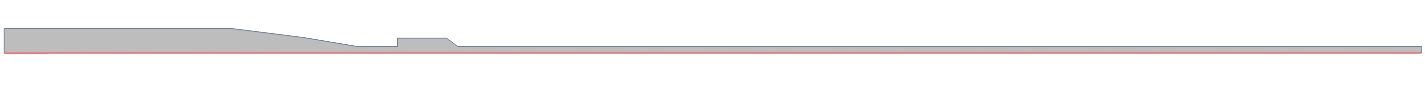
\includegraphics[width=15cm]{ostr-constelation-data/figures/ostr-coupled-3e-1mm-poly_Geometry Scene 1_cropped.png}};

    \node[inner sep=1.5pt,circle,fill=C0] (DV01) at (-6.28,-0.1) {}; % old: -6.28   new: -6.28
    \node[text width =1cm] (dv01 label) at (-6.28,-0.75) {\centering DV01\\};
    \draw[C0,-latex]  (dv01 label) -- (DV01);

    %\node[inner sep=1.5pt,circle,fill=C1] (DV02) at (-3.84,-0.1) {};
    %\node[text width =1cm] (dv02 label) at (-3.84,-0.75) {\centering DV02\\};
    %\draw[C1,-latex]  (dv02 label) -- (DV02);

    \node[inner sep=1.5pt,circle,fill=C2] (TS01) at (-0.30,-0.1) {};  % old: -2.2213   new: -0.30
    \node[text width =1cm] (ts01 label) at (-0.30,-0.75) {\centering TS01\\};
    \draw[C2,-latex]  (ts01 label) -- (TS01);

    \node[inner sep=1.5pt,circle,fill=C3] (TS02) at (2.55,-0.1) {};  % old: 1.019137   new: 2.55
    \node[text width =1cm] (ts02 label) at (2.55,-0.75) {\centering TS02\\};
    \draw[C3,-latex]  (ts02 label) -- (TS02);

    \node[inner sep=1.5pt,circle,fill=C4] (TS03) at (5.40,-0.1) {};  % old: 4.26  new: 5.40
    \node[text width =1cm] (ts03 label) at (4.26,-0.75) {\centering TS03\\};
    \draw[C4,-latex]  (ts03 label) -- (TS03);

    \node[inner sep=1.5pt,circle,fill=C5] (TS04) at (7.4,-0.1) {};  % old: 7.4   new: 7.4
    \node[text width =1cm] (ts04 label) at (7.4,-0.75) {\centering TS04\\};
    \draw[C5,-latex]  (ts04 label) -- (TS04);




\end{tikzpicture}




\end{document}